\documentclass[../NormediProgetto.tex]{subfiles}

\begin{document}
	
% NORME DI PROGETTO - Verifica
	
	
\section{Verifica}

\subsection{Scopo}
Il processo di verifica ha lo scopo di accertare che non vengano introdotti errori nel prodotto a seguito dello svolgimento delle attività dei processi.

\subsection{Descrizione}

Il processo di verifica viene istanziato per ogni processo in esecuzione, qualora esso raggiunga un livello di maturità significativo o vi fossero modiche sostanziali al suo stato. Per ogni processo viene verificata la qualità dello stesso e dei suoi prodotti. Ognuno dei periodi descritti nel PP produce degli esiti diversi, dunque le procedure di verifica saranno specializzate per ognuno di essi. Gli esiti delle attività di
verifica sono riportati in un'appendice dedicata nel PQ (§C). 
In relazione alle attività di verifica, il gruppo si riferisce alle metriche descritte in §3.3 di questo documento. Il processo di verifica agisce su:
\begin{itemize}
	\item \textbf{Processi}: l'esecuzione dei processi viene monitorata e documentato secondo le metodologie indicate dallo standard \glossario{ISO/IEC 15504}{ISO/IEC 15504} illustrato in appendice §A.1 del PQ;
	\item \textbf{Prodotti}: la verifica dei prodotti assume connotazioni differenti a seconda della tipologia di prodotto in esame: per i documenti si prediligono tecniche di analisi statica, per il software tecniche di analisi dinamica, di seguito approfondite.
\end{itemize}

\subsection{Analisi}

\subsubsection{Analisi statica}

L’analisi statica è una tecnica che permette di individuare anomalie all’interno di documenti e codice sorgente durante tutto il loro ciclo di vita. Si può realizzare tramite due tecniche diverse:

\begin{itemize}
	\item \textbf{Walkthrough:} viene svolta effettuando una lettura a largo spettro. Si tratta di un’attività collaborativa onerosa e poco efficiente. Essa viene utilizzata principalmente durante la fase iniziale del progetto, in cui non tutti i membri del gruppo hanno piena padronanza e conoscenza delle NP e del PQ. Tramite analisi \textit{Walkthrough} è possibile stilare una lista di controllo contenente gli errori più comuni;
	
	\item \textbf{Inspection:} viene svolta una lettura mirata e strutturata, volta a localizzare gli errori segnalati nella lista di controllo con il minor costo possibile. Con l'incremento dell'esperienza, la lista di controllo viene progressivamente estesa rendendo l’ispezione via via più efficace.
\end{itemize}

Il gruppo utilizza entrambe le tecniche di analisi statica. Seguono le liste di controllo per gli errori comuni relativi a documentazione e codice.

\subsubsection*{Lista di controllo per la documentazione}

\begin{longtable}{| p{5cm} |p{8cm} |}
	\caption {Tabella errori comuni - documentazione} \\
	\hline  
	\textbf{Anomalia} & \textbf{Descrizione}  \\ 
	\hline 
	Comandi \LaTeX deprecati & Uso di comandi \LaTeX successivamente ridefiniti \\ 
	\hline 
	Date & Formato delle date non conforme alle NP  \\ 
	\hline 
	Elenchi puntati & Elenchi puntati non conformi alle NP  \\ 
	\hline 
	Errori grammaticali & Errori grammaticali non rilevati dal controllo automatico dell'editor  \\ 
	\hline 
\end{longtable} 

\subsubsection*{Lista di controllo per il codice}

\begin{longtable}{| p{5cm} |p{8cm} |}
	\caption {Tabella errori comuni - codice} \\
	\hline  
	\textbf{Anomalia} & \textbf{Descrizione}  \\ 
	\hline 
	Classe non delimitata & Omissione di parentesi graffa di chiusura o di punto e virgola al termine di una classe \\ 
	\hline 
	Funzione non delimitata & Omissione di parentesi graffa di chiusura o di punto e virgola al termine di una funzione  \\ 
	\hline 
	Statement non delimitato & Omissione di punto e virgola al termine di uno statement \\ 
	\hline 
	Richiamo errato di variabili & Utilizzo di variabili già definite ma richiamate con errori di
	battitura  \\ 
	\hline 
\end{longtable} 

\subsubsection{Analisi dinamica}

L’analisi dinamica è una tecnica di analisi del prodotto software che richiede la sua esecuzione. Viene effettuata mediante dei test volti a verificare il funzionamento del prodotto e nel caso in cui vengano riscontrate anomalie ne permette l’identificazione. I test devono essere ripetibili, cioè deve essere possibile, dato lo stesso input nello stesso ambiente d'esecuzione, ottenere lo stesso output. Per ogni test devono dunque essere definiti i seguenti parametri:

\begin{itemize}
	\item \textbf{Ambiente d'esecuzione:} il sistema hardware e software sul quale verrà eseguito il test;
	\item \textbf{Stato iniziale:} lo stato iniziale dal quale il test viene eseguito;
	\item \textbf{Input:} l’input inserito;
	\item \textbf{Output:} l’output atteso;
	\item \textbf{Istruzioni aggiuntive:} ulteriori istruzioni su come eseguire il test e su come interpretare i risultati ottenuti.
\end{itemize}

I test verranno eseguite automaticamente ad ogni commit effettuato tramite l'integrazione continua attuata grazie a \textit{Travis CI}, mentre la copertura del codice verrà assicurata dal servizio web \textit{codcov.io}, anch'esso integrabile con Github, che permette di ottenere viste immediate circa la copertura del codice dopo ogni build. Tali test si differenziano tra loro secondo quanto illustrato nei paragrafi che seguono; una
trattazione più approfondita, assieme al tracciamento, è reperibile nel PQ (Appendice §B).

\subsection{Procedure}

\subsubsection{Verifica dei documenti}

\begin{enumerate}
	\item Assegnazione della issue di verifica ad un \textit{Verificatore} da parte del \textit{Responsabile di progetto};
	
	\item Controllo degli errori comuni secondo checklist;
	
	\item Lettura dei contenuti e correzione degli errori logici e sintattici;
	
	\item Tracciamento degli errori rilevati;
	
	\item Notifica dell'issue come \textit{verified} (precedentemente \textit{verify}).
\end{enumerate}

Segue il diagramma di flusso che riassume la procedura di verifica dei documenti:

\begin{figure}[H]
	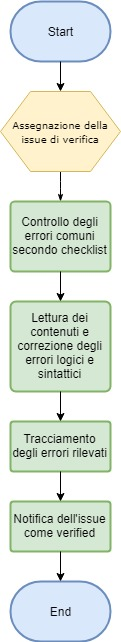
\includegraphics[scale=0.8]{verifica-documenti}
	\centering
	\caption{Diagramma della procedura di verifica dei documenti}
\end{figure}

\newpage

\subsubsection{Verifica del software}

La verifica del software avviene mediante tecniche di analisi dinamica, con la creazione di test automatici e tramite misurazioni apposite delle metriche illustrate in §3.3. Segue la procedura di verifica del software:

\begin{enumerate}
	\item Implementazione del codice;
	
	\item Commit del codice sul repository;
	
	\item Esecuzione della build;
	
	\item Esecuzione della suite di test;
	
	\item Esecuzione della build testata;
	
	\item Calcolo della copertura del codice e delle altre metriche pertinenti con relativa documentazione dei risultati.
\end{enumerate}

Segue il diagramma di flusso che riassume la procedura di verifica del software:

\begin{figure}[H]
	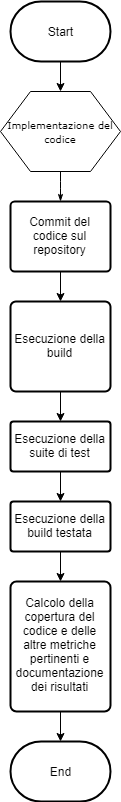
\includegraphics[scale=0.7]{verifica-software}
	\centering
	\caption{Diagramma della procedura di verifica del software}
\end{figure}

\subsubsection{Accertamento di qualità di prodotto}
Il controllo della qualità del prodotto viene garantito dai processi di verifica e di validazione, nonché dal rispetto delle norme di progetto.
\begin{itemize}
	\item \textbf{Verifica}: questo processo si occupa di accertare che l’esecuzione delle attività
	di processo siano corrette. Si applica ad ogni attività o risultato che fa progredire il progetto da una baseline alla successiva;
	\item \textbf{Validazione}: questo processo viene svolto come azione conclusiva per accertare
	che il prodotto rispecchi le aspettative utilizzando un metodo sistematico, disciplinato
	e quantificabile;
	\item \textbf{Rispetto delle norme}: il prodotto deve rispettare le norme e gli strumenti descritti dal
	presente documento.
\end{itemize}

\subsubsection{Accertamento di qualità di processo}
La qualità di un processo viene raffinata attraverso il miglioramento continuo indotto dal modello PDCA (Plan-Do-Check-Act) che apporta in modo incrementale qualità sempre maggiore. Ogni attività del modello deve avere una scrupolosa pianificazione ed un’ottima strategia di verifica che, all’interno di una determinata attività, permetta una serie di iterazioni fino al raggiungimento di un grado di qualità accettabile per poter procedere ad un ulteriore incremento. Per poter parlare di un possibile miglioramento della qualità di un processo, bisogna quantificare la qualità studiandone caratteristiche di interesse. Ciò viene attuato sulla base dello standard SPICE approfondito in §A.1 del PQ.

\subsection{Test}

La tecnologia utilizzata per la realizzazione dei test è \textit{Google Test}, approfondita in §4.7.4 di questo documento. 
Di seguito vengono riportate le tipologie di test eseguite sul software prodotto, le cui specifiche sono dettagliate nell'appendice §B del PQ:

\begin{itemize}
    \item \textbf{Test di unità:} i test di unità hanno l'obiettivo primario di isolare la parte più piccola di software testabile, indicata col nome di unità, per stabilire se essa funziona esattamente come previsto. Ogni test di unità deve avere almeno un metodo correlato da testare e deve rispettare la seguente nomenclatura:
    
    \begin{center}
        TU[Progressivo]
    \end{center}

    \item \textbf{Test di integrazione:} i test di integrazione valutano due o più unità già sottoposte a test come fossero un solo componente, testando le interfacce presenti tra loro al fine di rilevare eventuali inconsistenze. Risulta conveniente testare le unità a coppie aggiungendone gradualmente altre, così da poter rendere immediatamente tracciabile l'origine delle anomalie. Ogni test d'integrazione deve avere almeno un paio di componenti correlate da testare e rispettare la seguente nomenclatura:
    
    \begin{center}
        TI[Progressivo]
    \end{center}
    
    \item \textbf{Test di regressione:} i test di regressione devono essere eseguiti ad ogni modifica di un’\glossario{implementazione}{implementazione} all'interno del sistema. A tal fine è necessario eseguire sul codice modificato i test esistenti, in modo da stabilire se le modifiche apportate hanno alterato elementi precedentemente funzionanti.
    
    \item \textbf{Test di sistema:} i test di sistema determinano la validazione del prodotto software finale e verificano dunque che esso soddisfi in modo completo i requisiti fissati. Ogni test di sistema deve avere un requisito correlato da testare e deve rispettare la seguente nomenclatura:
    
    \begin{center}
        TS[Tipologia][Importanza][Codice]
    \end{center}

    Dove Tipologia, Importanza e Codice sono dedotti dal requisito correlato che il test va a verificare.

    \item \textbf{Test di validazione:} il test di accettazione prevede il \glossario{collaudo}{collaudo} del prodotto in presenza del \glossario{proponente}{proponente} e, in caso di superamento di tale collaudo, consegue il rilascio ufficiale del prodotto sviluppato. Ogni test di validazione deve avere un requisito correlato da testare e deve rispettare la seguente nomenclatura:

    \begin{center}
        TV[Tipologia][Importanza][Codice]
    \end{center}

    Dove Tipologia, Importanza e Codice sono dedotti dal requisito correlato che il test va a verificare.

\end{itemize}

% NORME DI PROGETTO - Validazione

\section{Validazione}

\subsection{Scopo}
Il processo di validazione ha lo scopo di accertare se il prodotto software e relativa documentazione verificati sono conformi a quanto preventivato.

\subsection{Descrizione}
Concluso il processo di verifica, viene istanziato quello di validazione, in cui nuovi \textit{Verificatori} designati dal \textit{Responsabile} accertano che i risultati prodotti siano conformi agli obiettivi di qualità. Se l'esito del processo di validazione è positivo, il \textit{Responsabile di Progetto} provvede all'approvazione dei documenti e/o del software a lui sottoposti.

\noindent Questo processo consta di due principali attività:
\begin{itemize}
    \item Test di sistema e di validazione;
    \item Collaudo.
\end{itemize}

\noindent Le attività svolte nel processo di validazione sono dunque le seguenti:

\begin{itemize}
    \item Pianificazione dei test da eseguire e relativo tracciamento;
    
    \item Conduzione di test che stressino il software nei suoi punti critici, ovvero laddove è più probabile il verificarsi di errori;
    
    \item Verifica del soddisfacimento dei requisiti secondo le informazioni di tracciamento.
\end{itemize}

È compito dei \textit{Progettisti} definire la pianificazione e la progettazione dei test. Compito dei \textit{Verificatori} è invece eseguirli e tracciarne i risultati tramite gli strumenti a ciò preposti. Per garantire la dovuta imparzialità nell'esecuzione, chi esegue un determinato test è necessariamente un membro del gruppo che non lo ha progettato ed implementato. Ad ulteriore garanzia di indipendenza, è intenzione del gruppo concordare un incontro con il committente in cui effettuare i test di sistema e validazione.

\subsection{Procedure}

\subsubsection{Validazione dei documenti}

\begin{enumerate}
    \item Assegnazione della issue relativa alla validazione ad un \textit{Verificatore} da parte del \textit{Responsabile};
    
    \item Calcolo dell'indice Gulpease e confronto del valore ottenuto con i parametri di riferimento;
    
    \item Se i risultati rilevati vengono ritenuti soddisfacenti, il documento viene approvato.
\end{enumerate}
    
Segue il diagramma di flusso che riassume la procedura di validazione dei documenti:

\begin{figure}[H]
	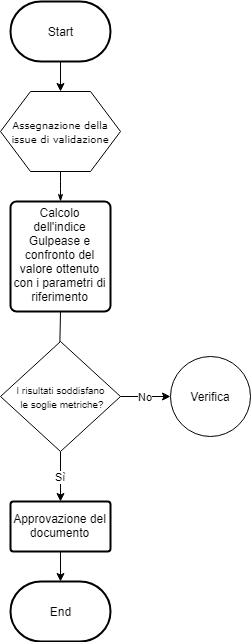
\includegraphics[scale=0.75]{validazione-documenti}
	\centering
	\caption{Diagramma della procedura di validazione dei documenti}
\end{figure}

\subsubsection{Validazione del software}

\begin{enumerate}
    \item Esecuzione dei test di sistema;
    
    \item Esecuzione dei test di validazione.
\end{enumerate}
    
Segue il diagramma di flusso che riassume la procedura di validazione del software:

\begin{figure}[H]
	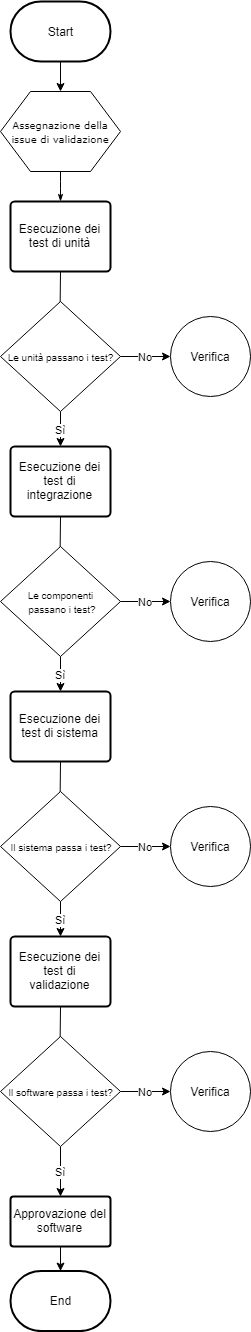
\includegraphics[scale=0.5]{validazione-software}
	\centering
	\caption{Diagramma della procedura di validazione del software}
\end{figure}

\subsection{Collaudo}

A seguito di una soddisfacente verifica e validazione del software, è intenzione del gruppo concordare un incontro con il Committente per eseguire un collaudo.

\end{document}